\documentclass{article}

% Language setting
% Replace `english' with e.g. `spanish' to change the document language
\usepackage[english]{babel}

% Set page size and margins
\usepackage[a4paper,top=2cm,bottom=2cm,left=3cm,right=3cm,marginparwidth=1.75cm]{geometry}

% Useful packages
\usepackage{amsmath}
\usepackage{graphicx}
\usepackage[colorlinks=true, allcolors=blue]{hyperref}
\usepackage{listings}
% \usepackage{bera}% optional: just to have a nice mono-spaced font
\usepackage{xcolor}
\usepackage{makeidx}

\usepackage{authblk}
\usepackage{blindtext}

\colorlet{punct}{red!60!black}
\definecolor{background}{HTML}{EEEEEE}
\definecolor{delim}{RGB}{20,105,176}
\colorlet{numb}{magenta!60!black}

\lstdefinelanguage{json}{
    basicstyle=\normalfont\ttfamily,
    numbers=left,
    numberstyle=\scriptsize,
    stepnumber=1,
    numbersep=8pt,
    showstringspaces=false,
    breaklines=true,
    frame=lines,
    backgroundcolor=\color{background},
}


\NewDocumentCommand{\codeword}{v}{
\texttt{\textcolor{blue}{#1}}
}

\title{\textbf{A bibliographic analysis of LiDAR Odometry and Mapping literature} \\ \textit{\normalsize{Social Network Analysis Project report}}}
\author{Federico Gavioli}
\affil{\textit{federico.gavioli@unimore.it}}
\date{June 27, 2025}

\begin{document}
\maketitle

\begin{abstract}
Lidar odometry is a fundamental technique in the field of autonomous navigation, playing a critical role in enabling an accurate motion estimation. Unlike GPS, which can suffer from signal loss or high inaccuracy in urban or indoor environments, LiDAR-based sensors offer an on-edge, resilient and stable solution for motion estimation. As the demand for reliable self-driving vehicles, drones, and robotic platforms continues to grow, an accurate and robust on-edge estimate is a crucial element to the system's safety. In this report, I present a bibliographic analysis of the LiDAR odometry literature. The analysis is carried out with the bibliometrix package of the R scripting language.
\end{abstract}

\section{Introduction}
Lidar odometry involves aligning point clouds to estimate the motion of the sensor (and thus, of the robot) over time, allowing for real-time localization and mapping of the surrounding environment.

My personal research focuses on high performance embedded platforms for autonomous systems, particularly by studying hardware acceleration and offloading solutions for on-edge sensor processing.

In this report, I will analyze the state of the art papers in lidar odometry This will help me understand the key methods, algorithms and performance requirements of future autonomous applications, making my research on autonomous platforms relevant to real-world scenarios. By conducting this literature review and social network analysis of this research community, I aim to uncover the most influential works and authors in this field and to understand how the focus of the research has shifted over time. This will provide a solid foundation for my future work in hardware offloading solutions for autonomous embedded systems.

\section{Dataset}
Given the topic of this bibliographic analysis, I have chosen to focus on the broader field of lidar odometry. The dataset used in this analysis is a collection of bibliographic records that includes papers, articles, and conference proceedings relevant to lidar odometry.

\subsection{Dataset collection}
The bibliographic dataset obtained via Web of Science, a major abstract and citation database. It was chosen for its comprehensive coverage of scientific literature and because, unlike Scopus, it allows the export of citation for each article.

\vspace{1em}
\begin{lstlisting}[language=json,label={lst:query},caption={Web of Science query used to collect the dataset},captionpos=b,firstnumber=1,frame=single]
lidar odometry (All Fields)
and Radar (Exclude)
and Article or Proceeding Paper (Document Types)
\end{lstlisting}

The query used to collect the data (Listing \ref{lst:query}) contains the \codeword{lidar odometry} terms, which are intentionally broad in order to capture a wide range of literature works. The query is subsequently refined to filter only on articles and conference papers and to remove false positives related to radar odometry, which is out of the topic of this analysis.

The dataset was finally exported in BibTeX format including all available metadata from Web of Science. Since Web of Science does not allow exporting more than 500 records in a single file, it was exported in multiple files, which are then merged into a single final dataset for the analysis.

\subsection{Dataset overview}
The bibliographic analysis was carried out in the R language using the bibliometrix\cite{bibliometrix} package and its web interface, biblioshiny\cite{biblioshiny}.

\begin{figure}[!htbp]
    \centering
    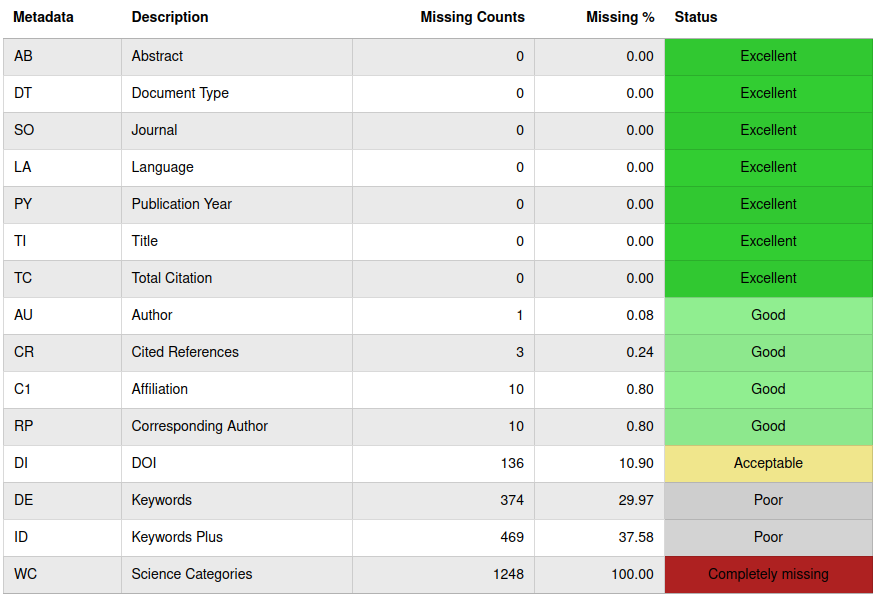
\includegraphics[width=1.0\textwidth]{img/import.png}
    \caption{Dataset import results and missing data.}
    \label{fig:import}
\end{figure}

As we can see from Figure \ref{fig:import}, the dataset contains a total of 1248 records. The \codeword{Author's Keywords} and \codeword{Keywords Plus} fields are missing from a significant number of records (respectively 29.97\% and 37.58\%). By further analyzing the data, we notice that the \codeword{Keywords Plus} field contains 355 unique keywords, while the \codeword{Author's Keywords} field contains 2177 instead, so the latter will be used for the analysis as it is considered more informative.

The dataset covers publications over a period of 19 years, from 2006 to 2025, with documents in the LiDAR odometry field coming from 494 journals and conferences. The paper count per year increased significantly in the last few years, with an annual grow rate of 27\%. This further confirms the rising relevance of the research field, as many researchers started to address this problem in the global rise of autonomous systems research.

The most cited papers in the dataset are shown in Table \ref{table:most_cited}. We can that the most influential works in the field are foundational LiDAR odometry and mapping techniques like LeGO-LOAM\cite{legoloam}, LIO-SAM\cite{liosam} and FAST-LIO2\cite{fastlio}.

\begin{table}[h!]
    \centering
    \begin{tabular}{||c c c c c c||}
        \hline
        \textbf{Paper} & \textbf{1st Author} & \textbf{Year} & \textbf{Venue} &  \textbf{Total Citations} & \textbf{TC per Year} \\ [0.5ex]
        \hline\hline
        LeGO-LOAM & Tixiao Shan & 2018 & IROS & 1405 & 175.63 \\
        \hline
        SemanticKITTI & Jens Behley & 2019 & ICCV & 1400 & 200.00 \\
        \hline
        LIO-SAM & Tixiao Shan & 2020 & IROS & 1151	& 191.83 \\
        \hline
        FAST-LIO2 & Wei Xu & 2022 & T-RO & 644	& 161.00 \\
        \hline
        Low-drift RT Odometry & Ji Zhang & 2017 & AUTON & 558 & 62.00 \\
        \hline
    \end{tabular}
    \caption{Most cited papers in the dataset}
    \label{table:most_cited}
\end{table}

In order to remove non-relevant papers, I have filtered the dataset to include only articles and conference papers with at least one citation per year. This brings the dataset size down to a total of 669 records.

\section{Questions and Analysis}
After getting a general feel for the available data, I have identified some questions which are interesting to guide the network analysis of this community.

% Q1
\subsection{Which authors are most central in advancing LiDAR odometry research? How are they connect and interact between each other?}

To answer this question, we will analyze the co-authorship network of the authors in the dataset. The most central authors can be highlighted by calculating a centrality measure of nodes the network. For this analysis, I decided to use the eigenvalue centrality metric, as it better captures the influence of a node in the network, taking into account not only the number of connections but also the importance of the connected nodes.

\begin{figure}[!htbp]
    \centering
    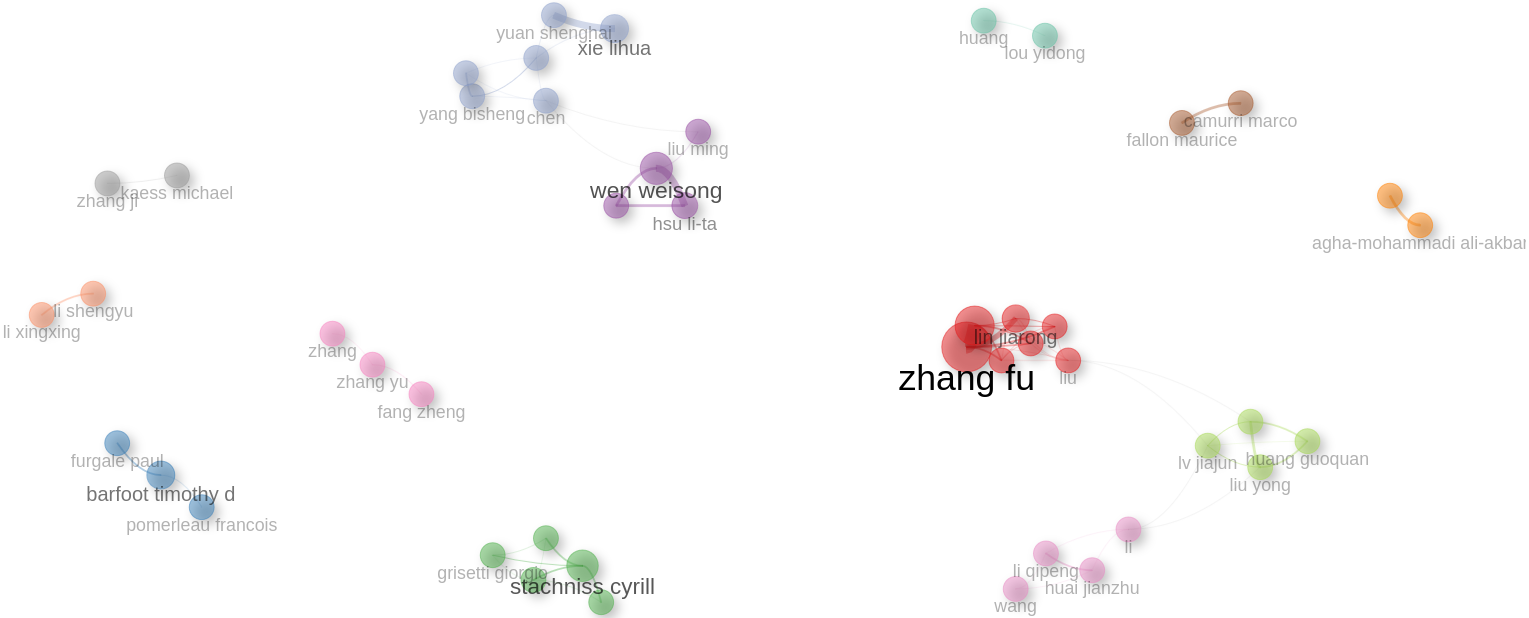
\includegraphics[width=1.0\textwidth]{img/coauth_network.png}
    \caption{Co-authorship network of LiDAR Odometry authors.}
    \label{fig:coauth_network}
\end{figure}

The resulting network (Figure \ref{fig:coauth_network}) shows the co-authorship relationships between institutions in the LiDAR odometry research area. The size of the nodes represents the eigenvalue centrality of each institution, while the edges represent the co-authorship relationships between them. We can immediately notice that the graph is quite disconnected, with several isolated nodes and small clusters of institutions working together. This is understandable as the topic is quite new and collaborations are yet to be established between different research groups. Nevertheless, we can identify some clusters of institutions working together:
\begin{itemize}
    \item \textbf{Zhang Fu} connects a small cluster of Chinese researchers. However, it's important to note that this is likely a false positive, as the name identifies two different researchers in different Chinese universities working on the same topic, and to my understanding Biblioshiny has no way to disambiguate between them.
    \item \textbf{Cyrill Stachniss}, from the University of Bonn, is central to a fruitful collaboration between European universities. In its cluster, we can also find Giorgio Grisetti, an Italian researcher at the Sapienza University of Rome.
    \item \textbf{Timothy Barfoot} leads a small cluster of Canadian researchers, including the University of Toronto and the University of Laval.
\end{itemize}

From this analysis, we can conclude that the LiDAR odometry research area is still quite fragmented, with several isolated institutions and small clusters of researchers working together. However, identified some key researchers and institutions that are actively working together to advance the field and are likely to have a significant impact on its future development.


% Q2
\subsection{How has the focus on this research topic shifted over time?}
To perform a thematic analysis of the research area, we will first need to analyze how the paper production density over time. We can assume that peaks in the number of publications correspond to shifts in the research focus, as they indicate a growing interest in a specific topic.

\begin{figure}[!htbp]
    \centering
    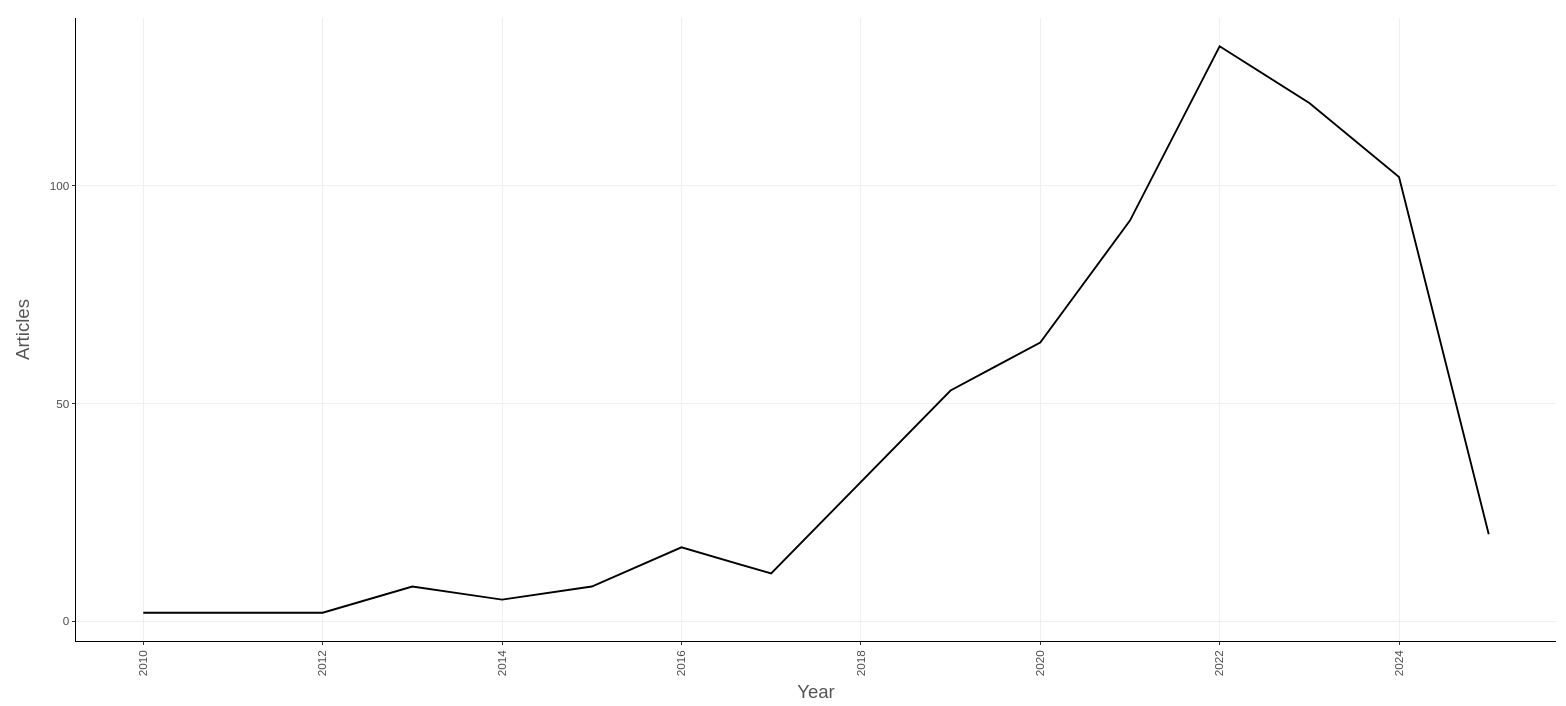
\includegraphics[width=1.0\textwidth]{img/paper_production.png}
    \caption{Papers published over time.}
    \label{fig:paper_production}
\end{figure}

We can se from the graph in Figure \ref{fig:paper_production} that the number of publications has three peaks, respectively in 2016, 2018 and 2022. We can use this peaks to split the dataset into four time periods to perform a thematic evolution analysis of the papers published in each period.

\begin{figure}[!htbp]
    \centering
    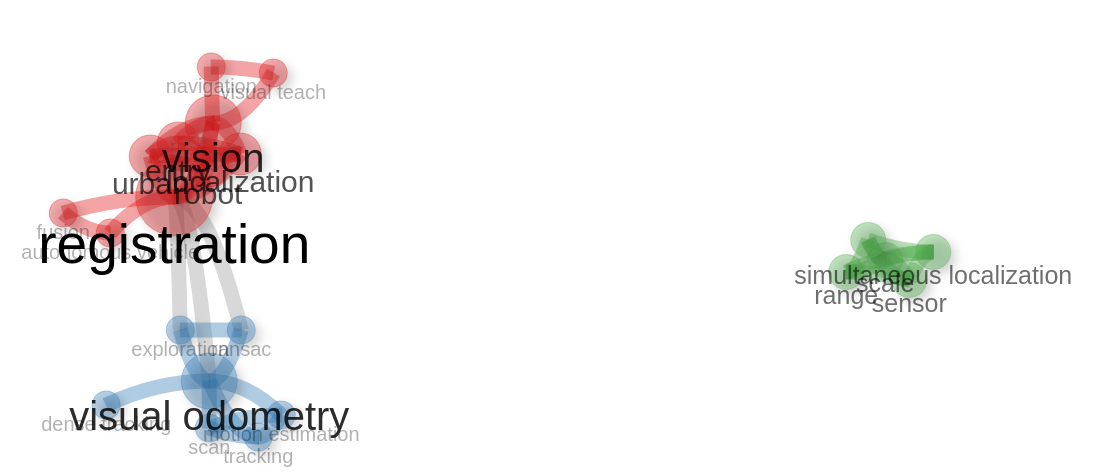
\includegraphics[width=1.0\textwidth]{img/topics_until2016.png}
    \caption{Topics until 2016.}
    \label{fig:topics_until2016}
\end{figure}

In Figure \ref{fig:topics_until2016}, we can see the topics of the papers published until 2016. The most relevant keywords are \codeword{registration}, \codeword{visual odometry} and \codeword{sensor}. This is consistent with the fact that the field was still in its early stages, with researchers focusing on foundational techniques for LiDAR odometry and mapping.

\begin{figure}[!htbp]
    \centering
    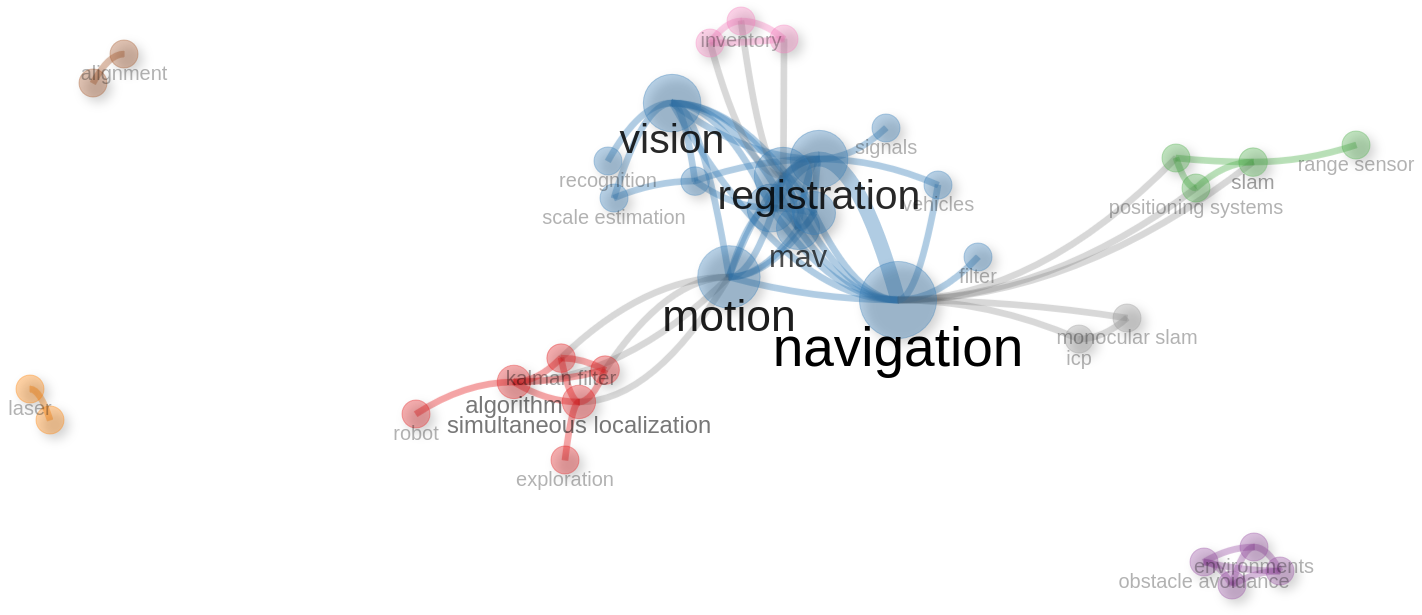
\includegraphics[width=1.0\textwidth]{img/topics_2017_2018.png}
    \caption{Topics between 2017 and 2018.}
    \label{fig:topics_2016_2018}
\end{figure}

In Figure \ref{fig:topics_2016_2018}, we can see the topics of the papers published between 2017 and 2018. The most relevant keywords are moving closer to the applicative domain of lidar odometry techniques, with keywords like \codeword{navigation}, \codeword{motion} and \codeword{MAV} (Micro Aerial Vehicle). This shift highlights the transfer of the research interest to the deployment of lidar odometry solutions to real applications.

\begin{figure}[!htbp]
    \centering
    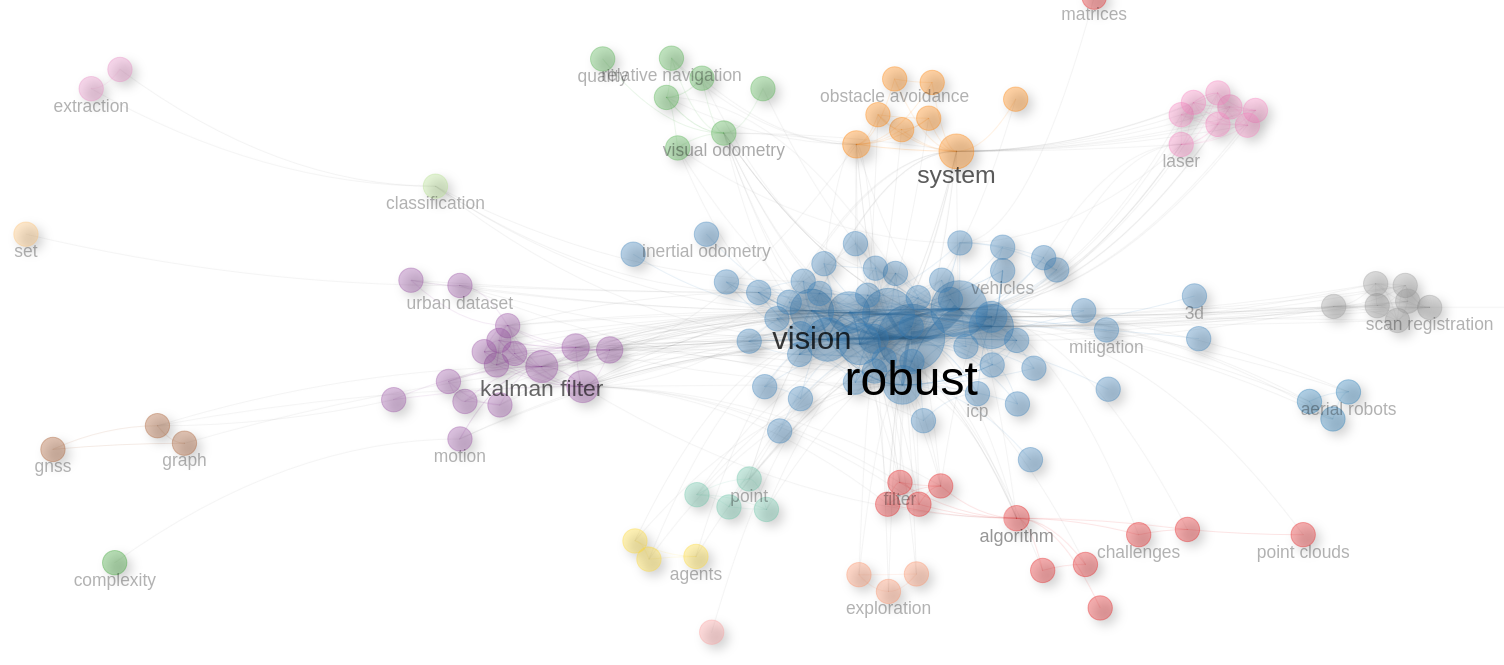
\includegraphics[width=1.0\textwidth]{img/topics_2019_2022.png}
    \caption{Topics between 2019 and 2022.}
    \label{fig:topics_2019_2022}
\end{figure}

In Figure \ref{fig:topics_2019_2022}, we can see the topics of the papers published between 2019 and 2022. Another shift in the research focus is evident, with keywords like \codeword{robust}, \codeword{kalman filter} and \codeword{system} becoming more relevant. This indicates a growing interest in finding not only an accurate solution for lidar odometry, but also a robust and reliable one. The presence of the \codeword{kalman filter} keyword also suggests that a KF-based odometry is becoming more popular in the field, likely due to their ability to provide a more stable and noise-resistant estimate.

\begin{figure}[!htbp]
    \centering
    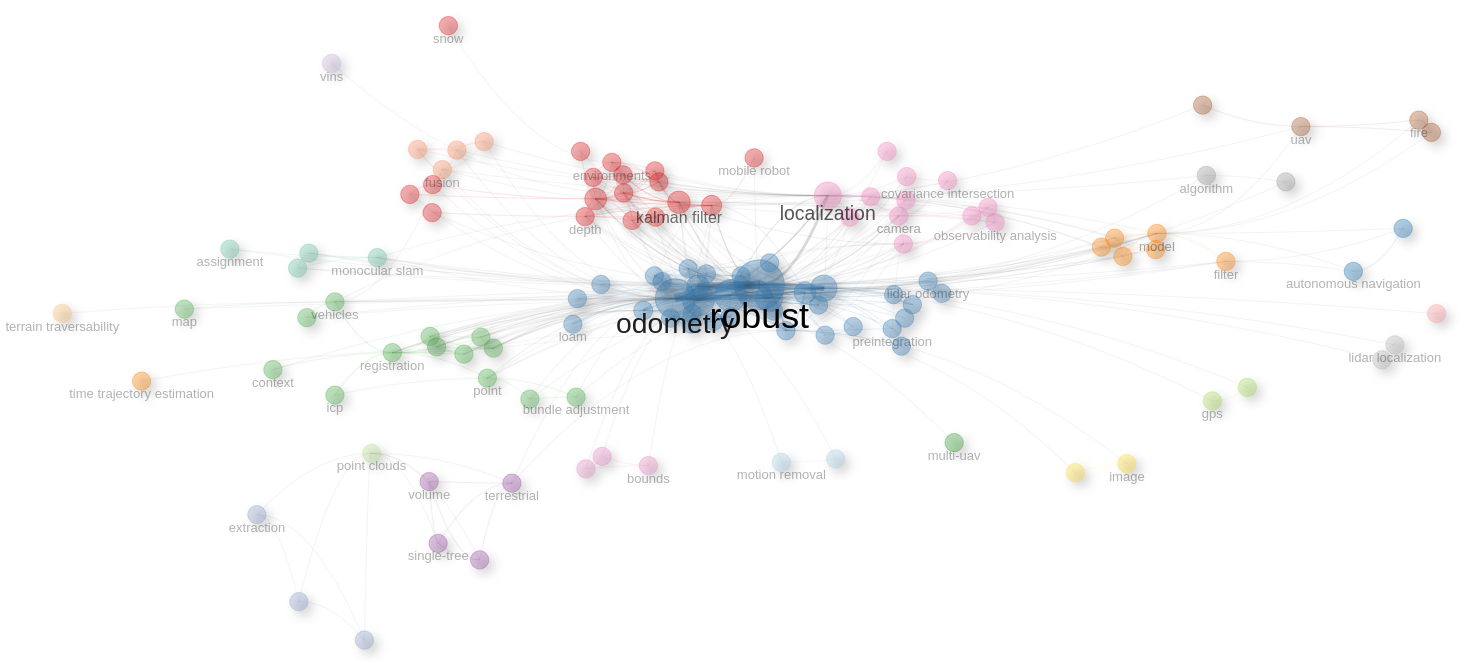
\includegraphics[width=1.0\textwidth]{img/topics_2023_2025.png}
    \caption{Topics between 2023 and 2025.}
    \label{fig:topics_2023_2025}
\end{figure}

Finally, we can analyze the topics of the papers between 2023 and 2025, which are shown in Figure \ref{fig:topics_2023_2025}. The is becoming more and more fragmented, with several subfields emerging. This is due to the topic becoming more mature, with researchers focusing on specific aspects of the topic, like the 3D \codeword{localization} problem, the deployment on \codeword{terrestrial} vehicles or sensor \codeword{fusion}, integrating other sensors in the odometry pipeline.

\section{Conclusions}
The thematic analysis reveals that the focus of LiDAR odometry research has shifted from foundational methods and sensor registration to more robust, application-oriented solutions, with increasing attention to robustness and deployment in specific applicative scenarios. This is consistent with the growing interest in autonomous systems and the need for reliable and accurate motion estimation solutions. I now have valuable pointers to research works and topics to explore to make my research on hardware offloading solutions more effective and relevant to this quickly developing field.

\bibliographystyle{plain}
\bibliography{references}

\end{document}


% Questions:
% Which researchers or institutions are most central in advancing hardware offloading strategies?
%     - Si cerca di solito usare come grafo quello del co-authoring
% What are the major communities in this research area, and how do they interact?
%     - Attenzione al tipo di rete
% How has the focus shifted over time? Is software becoming prevalent?
%     - Fare diverse prove, magari tanti paper sono riferiti a un singolo periodo storico. Se dividi un periodo di 20 anni in blocchi da 5 non hai una distribuzione omogenea. Fare tanti tentativi.
% Are there "bridging" papers or authors that connect otherwise disconnected subfields (e.g., real-time OS design and deep learning deployment)?
%     -
